\begin{figure}
 \centering
 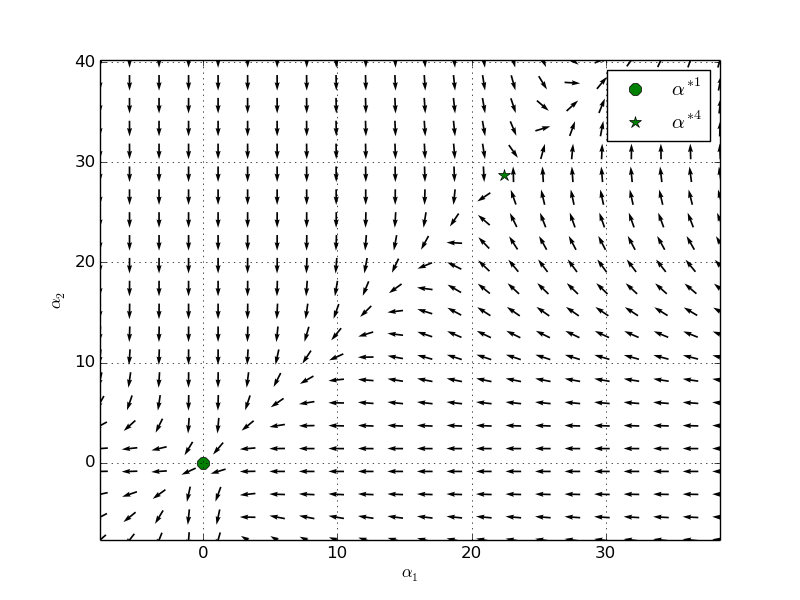
\includegraphics[scale = 0.7]{Python/plots/RG_flow/RG_flow3_2_6_0_2_0_1_0.png}
 \caption{Das Flussdiagramm für eine Lösung vom Typ \ref{Fall1b}. Der Fixpunkt 
  $\alpha^{*}_\text{vw}$ liegt im nicht-perturbativen Bereich. Die Parameter sind 
 $(\Nc,\Nd,\nfc,\nsc,\nfd,\nsd,\nfj,\nsj)=(3,2,6,0,2,0,1,0)$.}
 \label{fig:beta_QCDxdQCD:Sattelpunkt1}
\end{figure}
